\chapter{Sistemi discreti principali}

\section{Dinamica simbolica}
Sia $\Ac$ un alfabeto finito e sia $\Omega=\Ac^\N$. Imponiamo la topologia discreta su $\Ac$ e la topologia prodotto su $\Omega$. Per il teorema di Tychonoff segue dalla compattezza di $\Ac$ che $\Omega$ \`e compatto.\\
Lo spazio $\Omega$ \`e anche uno spazio metrico con distanza definita come segue:
\[d(\omega,\wt \omega)=\sum_{i=0}^\infty 2^{-i-1}\delta(\omega_i,\wt \omega_i),\]
dove $\delta(a,b)=\begin{cases}
1 & a\neq b\\
0 & a=b
\end{cases}$.

\begin{definition}[Shift]
Definiamo la mappa di \textbf{shift} come
\[\sigma:\funcDef{\Omega}{\Omega}{(\omega_i)_{i\in\N}}{(\omega_{i+1})_{i\in\N}}.\]
\end{definition}
\begin{remark}
La mappa di shift \`e continua perch\'e $2$-lipschitziana.
\end{remark}

Uno dei motivi principali per cui studiamo la mappa di shift \`e il seguente
\begin{proposition}[Lo shift \`e caotico]\label{ShiftECaos}
Consideriamo $\Ac=\cpa{1,\cdots, N}$, $\Omega=\Ac^\N$ con la metrica definita prima e $\sigma:\Omega\to\Omega$ lo shift, allora $\sigma$ \`e caotica su $\Omega$.
\end{proposition}
\begin{proof}[Dimostrazione. (Caotica per Devaney)]
Verifichiamo le tre condizioni:
\begin{enumerate}
\item Vogliamo mostrare che per ogni $\wt \omega$ e per ogni $\e>0$ esiste $\omega$ parola periodica \footnote{$\omega=sssss\cdots$ con $s\in \Ac^\ast$, cio\`e $s$ \`e una parola finita formata dai simboli in $\Ac$.} tale che $d(\omega,\wt \omega)<\e$. Fissati $\wt \omega$ e $\e$ basta prendere $s$ un opportuno troncamento di $\wt \omega$ (tanto la distanza \`e pesata molto sui simboli iniziali).
\item Gli aperti di $\Omega$ hanno come prebase i cilindri della forma
\[C(\omega,h,n)=\cpa{\wt \omega\in\Omega\mid \forall i\in\cpa{0,\cdots,n-1},\ \omega_{h+i}=\wt \omega_{h+i}}.\]
Vogliamo dunque mostrare che ogni $\omega^1,\ \omega^2\in\Omega$ e per ogni $h^1,h^2,n^1,n^2\geq 0$ esiste $m\in\N$ tale che
\[\sigma^m(C(\omega^1,h^1,n^1))\cap C(\omega^2,h^2,n^2)\neq \emptyset,\]
cerchiamo cio\`e $\wt \omega\in C(\omega^1,h^1,n^1)$ tale che $\sigma^m(\wt \omega)\in C(\omega^2,h^2,n^2)$. Basta porre che 
\[\rbar{\wt\omega}_{h^1+n^1-1}^{h^1}=\rbar{\omega^1}_{h^1+n^1-1}^{h^1}\quad\text{e}\quad\rbar{\wt\omega}_{m+h^2+n^2-1}^{m+h^2}=\rbar{\omega^2}_{h^2+n^2-1}^{h^2}\]
per un $m\gg h^1$.
\item Fissiamo $c\in (0,1)$. Fissati $\omega\in\Omega$ e $\e>0$ cerchiamo $\wt \omega\in B_\e(\omega)$ tale che esiste $m\in\N$ tale che $d(\sigma^m(\omega),\sigma^m(\wt \omega))>c$. Osserviamo che esiste $k_\e\in\N$ tale che se $\omega_i=\wt \omega_i$ per ogni $i\leq k_\e$ allora $d(\omega,\wt \omega)<\e$. Costruiamo allora $\wt \omega$ facendo s\`i che almeno i primi $k_\e$ simboli coincidano con quelli di $\omega$ e tale che tutti i successivi a un certo indice $m$ siano diversi tra le due successioni. Osserviamo allora che $d(\sigma^m(\omega),\sigma^m(\wt \omega))=\sum_{i\geq 0}2^{-i-1}\cdot 1=1>c$.
\end{enumerate}
\end{proof}
\begin{proof}[Dimostrazione. (Caotica per Entropia)]
Fissati $n,\e$ osserviamo che per ogni $\omega\neq \wt\omega$ esiste $k<n$ tale che $d(\sigma^k(\omega),\sigma^k(\wt \omega))>\e$ se e solo se esiste $i\in\cpa{0,\cdots, k_\e}$ tale che $\omega_{k+i}\neq \wt \omega_{k+i}$. Segue che se $S$ \`e $(n,\e)$-separato, la mappa di troncamento
\[\funcDef{S}{\cpa{1,\cdots, N}^{n+k_\e+1}}{s}{s\res{\cpa{0,\cdots, n+k_\e}}}\] \`e iniettiva. Poich\'e possiamo facilmente costruire un $S$ tale che la mappa sopra \`e bigettiva\footnote{Basta estendere arbitrariamente le stringhe dopo l'$(n+k_\e+1)$-esimo simbolo}, si ha che
\[\max\cpa{\# S\mid S\text{ \`e $(n,\e)$-separato}}\sim \#\cpa{1,\cdots, N}^{n+k_\e+1}\sim N^{n+k_\e},\]
da cui
\[h_{top}(\sigma)=\lim_{\e\to0^+}\limsup_{n\to+\infty} \frac{n+k_\e}n\log N=\log N.\]
\end{proof}

\section{Mappe di Poincar\'e}
Proviamo a capire quando un sistema di equazioni differenziali porta un'orbita a tornare vicino a se stessa.

\begin{definition}[Mappa di Poincar\'e]
Sia $M$ una variet\`a e sia $\Sigma$ una sua sottovariet\`a di codimensione 1 tale che esiste $U\subseteq \Sigma$ con la seguente propriet\`a:\\
se $P\in U$ allora esiste $\ol t>0$ tale che $t\in (0,\ol t)\implies \phi_t(P)\notin U$ e $\phi_{\ol t}(P)\in U$\footnote{$\ol t$ \`e l'istante del ``primo ritorno"}.\\
Definiamo la \textbf{mappa di Poincar\'e} come
\[P_U:\funcDef{U}{U}{(x,y)}{\phi_{\ol t}(x,y)}.\]
\end{definition}
\begin{remark}
Ponendo $P_\Sigma^0=id$ e
\[P_\Sigma^n=\under{n\text{ volte}}{P_\Sigma\circ\cdots\circ P_\Sigma}\]
stiamo definendo un sistema discreto $(\Sigma,P_\Sigma,\Z)$\footnote{$P_\Sigma^{-1}$ \`e definita perch\'e sono partito da un flusso e posso prendere tempi negativi in un flusso}.
\end{remark}

\begin{example}[Moto sul toro piatto]
Sia $T^2=\R^2/\Z^2$. Un moto geodetico sul toro (piatto) si pu\`o pensare come
\[t\mapsto \phi_t(x,y)=(x,y)+t(v_x,v_y)\mod{\Z^2}.\]
Sia $\Sigma=U=S^1=\quot{[0,1]\times\cpa0}{(0,0)\sim(1,0)}$. Per la geometria del toro questa sottovariet\`a di $T^2$ ha le propriet\`a richieste per definire la mappa di Poincar\'e (addirittura sappiamo che $\ol t=1/v_y$).\\
Esplicitamente troviamo che 
\[P_\Sigma:\funcDef{S^1}{S^1}{t}{t+\al \mod 1}\]
dove $\al=v_x/v_y$. Osserviamo che a meno di traslare modulo 1, tutte le orbite sono determinate dall'orbita di $0$.
\setlength{\leftmargini}{0cm}
\begin{itemize}
\item[$\boxed{\al\in\Q}$] Se $\al=\frac pq$ ridotta ai minimi termini allora $P_\Sigma^q(0)=0+p=0 \mod 1$ e le orbite sono periodiche.
\item[$\boxed{\al\in\R\bs\Q}$] Evidentemente non troviamo un'orbita periodica. \`E possibile mostrare che in realt\`a l'orbita \`e densa.
\end{itemize}
\setlength{\leftmargini}{0.5cm}
\end{example}


\begin{definition}[Semipiano di Poincar\'e]
Consideriamo la regione $[-1,1]\times [0,+\infty]\bs D^1$ e identifichiamo i lati come in figura
\begin{figure}[!htb]
    \centering
    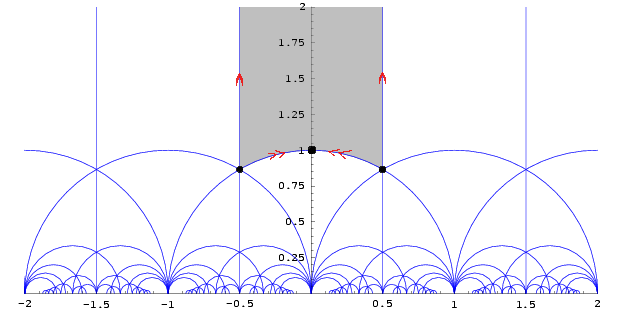
\includegraphics[width=9cm]{Immagini/ModularGroup-FundamentalDomain-01.png}
    \caption{Dominio fondamentale e qualche geodetica.}
    \label{SemipianoPoincare}
\end{figure}

\noindent
Le geodetiche sono le intersezioni dell'oggetto con rette verticali o semicirconferenze perpendicolari all'asse $x$.
Chiamiamo $\Mc$ questo spazio.
\end{definition}
\begin{example}[Geodetiche sul piano di Poincar\'e]
A parte le geodetiche corrispondenti a rette verticali, ogni geodetica che incontra la regione lo fa passando per l'asse $y$ (e quindi lo fa ad un certo angolo). Possiamo associare ad ogni coppia punto di $\Mc$ e angolo una geodetica di $\Mc$ (quella passante per il punto che incontra la verticale a quell'angolo)
\[\Mc\times S^1\ni ((x,y),\theta)\mapsto g_t((x,y),\theta).\]
Sia $\Sigma=\cpa{x=0,y>1}\times S^1$. \`E possibile definire $P_\Sigma$ e si da il caso che questa mappa di Poincar\'e \`e pi\`u facile da studiare rispetto al sistema originale.
\end{example}

\subsection{Sistemi continui caotici}
Le uniche nozioni di caos che abbiamo trattano i sistemi discreti, quindi se vogliamo studiare quando un sistema continuo manifesta un comportamento caotico con gli streumenti che abbiamo il procedimento standard \`e:
\begin{itemize}
\item Cercare $\Sigma$ di codimensione $1$ in $X$ che ammette $P:\Sigma\to\Sigma$ mappa di Poincar\'e.
\item Cercare $\Lambda\subseteq \Sigma$ positivamente invariante per $P$ su cui $P$ \`e topologicamente coniugata a $(\Omega,\sigma)$ dove $\sigma$ \`e lo shift.
\item Per la proposizione (\ref{ShiftECaos}) questo mostra che la mappa di Poincar\'e \`e caotica.
\end{itemize}


\section{Endomorfismi del cerchio e mappa di Bernoulli}
\begin{definition}[Endomorfismi lineari del cerchio]
Sia $m\in\R$, gli endomorfismi lineari del cerchio sono quelli della forma\footnote{Il caso $m=2$ restituisce la \textbf{mappa di Bernoulli}.}
\[T_m:\funcDef{S^1}{S^1}{x}{mx\mod 1}.\]
\end{definition}

\begin{example}[Punti fissi della mappa di Bernoulli]
Cerchiamo graficamente punti fissi e periodici di $T_2=T$
\begin{figure}[!htb]
    \centering
    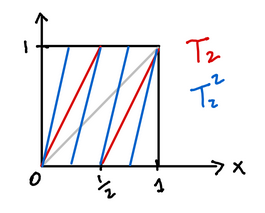
\includegraphics[width=5cm]{Immagini/Bernoulli.png}
    \caption{Un tipo di grafico utile la mappa di Bernoulli. In grigio troviamo l'identit\`a, in rosso $T_2$ e in blu $T_2^2$.}
\end{figure}

\noindent Evidentemente l'unico punto fisso \`e $0$ (dal disegno sarebbero $0$ e $1$, ma $0\equiv 1\mod 1$).\\
Cerchiamo ora punti con periodo minimo $2$, cio\`e
\[T^2(x)=x,\quad T(x)\neq x.\]
Ricordiamo che
\[T(x)=\begin{cases}
2x & 0\leq x< \frac12\\
2x-1 & \frac12\leq x<1
\end{cases}\implies
T^2=\begin{cases}
4x & 0\leq x<\frac14\\
2(2x)-1=4x-1 & \frac14\leq x<\frac12\\
2(2x-1)=4x-2 & \frac12\leq x<\frac34\\
2(2x-1)-1=4x-3 & \frac34\leq x<1
\end{cases}\]
Graficamente vediamo che ci sono due punti di periodo $2$, e questi sono $\frac13$ e $\frac23$. Osserviamo che i numeri della forma $3\ii\cdot 2^{-k}$ sono definitivamente periodici.\\
Cerchiamo i punti di periodo minimo $3$. Graficamente notiamo che sono $6$
    
\begin{figure}[!htb]
    \centering
    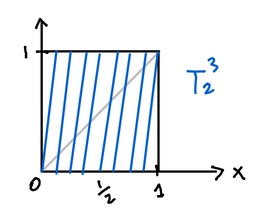
\includegraphics[width=5cm]{Immagini/Bernoulli_iterata.png}
    \caption{Rappresentazione grafica di $T^3_2$.}
\end{figure}

\noindent
In generale per come funzionano le iterate di $T_2$ si ha che il numero di punti di periodo (eventualmente non minimo) $n$ \`e $2^n-1$.
\end{example}

\begin{example}[Perdo il controllo]
Consideriamo la mappa
\[T:\funcDef{S^1}{S^1}{x}{10x \mod 1}.\]
Poniamo $\Ac=\cpa{0,\cdots,9}$ e $\Ac_n=\pa{\frac n{10},\frac{n+1}{10}}$ per $n\in\Ac$.\\
Sia $x\in \R\bs \Q$ e diamo la seguente mappa
\[\vp:x\mapsto(\omega_0,\omega_1,\cdots)\in \Ac^{\N}\]
dove $\omega_n=k\coimplies T^n(x)\in \Ac_k\coimplies \lfloor10 T^n(x)\rfloor=k$ e per ricorsione vediamo che $\omega_n$ \`e la $n$-esima cifra decimale di $x$, cio\`e
\[x=0.\omega_0\omega_1\omega_2\cdots.\]
Per rispondere ad una domanda del tipo ``$T^{1000}(x)\in \Ac_i?$" devo sapere la 1000-esima cifra di $x$. Se ora considero $y\in B_\e(x)$ al posto di $x$, le informazioni che avevamo su $x$ non dicono pi\`u nulla sul comportamento di $y$ oltre un certo passo\footnote{se $n>-\log_{10} \e$ la risposta a ``$T^{n}(x)\in \Ac_i?$" e quella a ``$T^{n}(y)\in \Ac_i?$" sono indipendenti.}.
\end{example}
    
\begin{remark}[Piccola parentesi statistica]
Sia $x=0.x_1x_2\cdots$ potremmo chiederci, fissata una cifra $k$ se
\[Prob\cpa{\lim_{N\to+\infty}\frac{\#\cpa{i\in \cpa{0,\cdots, N-1}\mid x_i=k}}{N}=\frac1{10}}=1\]
ed effettivamente \`e vero. Segue dunque che
\[Prob\cpa{\lim_{N\to+\infty}\frac{\#\cpa{i\in \cpa{0,\cdots, N-1}\mid x_i=k}}{N}=\frac1{9}}=0\]
anche se non \`e un insieme vuoto\footnote{per esempio posso fissare ogni nona cifra a $k$ e completare le altre con cifre a caso diverse da $k$.}.
\end{remark}

\begin{example}[Espansione binaria tramite la mappa di Bernoulli]
Sia $T_2:S^1\to S^1$, $T_2(x)=2x\mod 1$.\\
Sia $I_0=[0,\frac12)$, $I_1=[\frac12,1)$ e $\Omega=\cpa{0,1}^\N$. Consideriamo la mappa $\vp:S^1\to \Omega$ data da:
\[x\mapsto (\omega_0(x),\omega_1(x),\cdots),\quad \omega_i(x)=\begin{cases}
0 & T^i(x)\leq \frac12\\
1 & T^i(x)\geq\frac12
\end{cases}\]
Osserviamo che $\sigma\circ \vp=\vp\circ T_2$ ma $\vp$ non \`e un omeomorfismo (o ben definita\footnote{potremmo imporre di considerare solo i rappresentanti in $[0,1)$ e definire $\omega_i(x)=1$ se $T^i(x)=1/2$, ma queste scelte andrebbero a violare la surgettivit\`a di $\vp$ e la continuit\`a in generale.}), infatti
\[\vp\ii(1,0,0,0,\cdots)=\cpa{\frac12}=\vp\ii(0,1,1,1,1,\cdots).\]
Quello che sta succedendo che abbiamo trovato due serie della seguente forma che convergono allo stesso valore
\[x=\sum_{i\geq 0}\frac{\omega_i(x)}{2^{i+1}}.\]
\end{example}

\begin{example}
La mappa $T(x)=2x\mod 1$ \`e caotica nel senso di Devaney.
\begin{enumerate}
\item Le orbite periodiche corrispondono alle classi dei numeri razionali, i quali sono densi in $[0,1]$
\item suddividiamo $S^1=[0,1]/0\sim 1$ in intervalli lungo i razionali con denominatore pari ad una potenza di 2 (per esempio $\Jc_2=\cpa{[0,1/4], [1/4, 1/2], [1/2, 3/4], [3,4,1]}$). Dopo un opportuno numero di suddivisioni, esister\`a un $n$ per il quale un intervallo di $\Jc_n$ \`e interamente contenuto in $U$. Allora $T^n(U)=S^1$ e quindi in particolare $T^n(U)\cap V\neq \emptyset$, cio\`e $T$ \`e topologicamente transitiva.
\item Sia $x\in S^1$. Fissiamo $\e>0$ e sia $k$ un intero tale che $2\ii<\e$. Notiamo che in $B_\e(x)$ esiste un $y$ che coincide con $x$ definitivamente, per esempio possiamo considerare $x$ dove nell'espasione in base 2 abbiamo invertito la $(k+1)$-esima cifra. In tal caso $T^k(x)$ e $T^k(y)$ differiscono nella prima cifra ma coincidono nella seconda, quindi $d(T^k(x),T^k(y))= 1/2>1/4$, quindi se scegliamo $c=1/4$ abbiamo la dipendenza sensibile dai dati iniziali.
\end{enumerate}
\end{example}


\section{Mappa Logistica e Tenda}
\subsection{Mappa logistica} 
\begin{definition}[Mappa logistica]
Una funzione continua $T_\la:[0,1]\to[0,1]$ si dice \textbf{logistica} se \`e della forma\footnote{Le restrizioni $0\leq \la\leq 4$ servono per garantire che effettivamente $[0,1]$ sia il codominio.}
\[T_\la(x)=\la x(1-x),\quad 0\leq \la\leq 4.\]
\end{definition}

\begin{figure}[!htb]
    \centering
    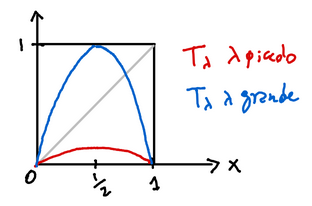
\includegraphics[width=6cm]{Immagini/Logistica.png}
    \caption{Rappresentazione di due mappe logistiche.}
\end{figure}

\subsubsection{Derivata}
La derivata di $T_\la(x)=\la x(1-x)$ \`e
\[T'_\la(x)=\la-2\la x.\]
Segue che $T_\la$ ha massimo in $1/2$.
\subsubsection{Punti fissi}
I punti fissi di $T_\la$ sono le soluzioni di
\[\la x(1-x)=x\coimplies x((\la-1)-\la x)=0,\]
cio\`e $0$ e $1-\la\ii$. Notiamo per\`o che il secondo punto fisso \`e rilevante solo se $1-\la\ii\in [0,1]$, cio\`e solo se $\la\geq 1$.\\
Calcoliamo quando questi punti fissi sono iperbolici:
\[T'_\la(0)=\la.\]
Per $\la<1$ si ha che $0$ \`e iperbolico attrattivo e che per $\la>1$ \`e iperbolico repulsivo.\\
Se $\la=1$ allora i due punti fissi coincidono e sono non iperbolici.
\[T'_\la(1-\la\ii)=2-\la.\]
Segue che $1-\la\ii$ \`e iperbolico attrattivo se $\la\in (1,3)$, iperbolico repulsivo se $\la\in (3,4]$ e non iperbolico per $\la\in\cpa{1,3}$.
Studiamo ora i casi di $\la=1$ e $\la=3$:
\setlength{\leftmargini}{0cm}
\begin{itemize}
\item[$\boxed{\la=1}$] Calcoliamo che $T_\la''(x)=-2\la<1$, quindi, poich\'e $T_\la'(0)=\la=1$ per il criterio per punti non iperbolici (\ref{CriterioPuntiNonIperboliciDerivataPositiva}) si ha che $0$ \`e attrattivo.
\item[$\boxed{\la=3}$] Il questo caso $1-\la\ii=2/3$, inotlre $T'(x)=3-6x$, $T''(x)=-6$ e $T'''(x)=0$. Segue che $ST(x)=0-\frac32(6/(3-6x))^2<0$, in particolare $ST(2/3)<0$ e quindi \`e un punto fisso attrattivo per il criterio per punti non iperbolici con derivata $-1$ (\ref{CriterioPuntiNonIperboliciDerivataNegativa}).
\end{itemize}


\subsubsection{Diagramma di biforcazione}
Osserviamo che 
\[T_\la^2(x)=\la(\la x(1-x))(1-\la x(1-x))=\la^2 x(1-x)(1-\la x(1-x)).\]
\noindent
Notiamo graficamente (Figura \ref{LogisticaIterata}) che in corrispondenza di $\la=3$ passiamo da una soluzione a due:
\begin{gather*}
\la^2 x(1-x)(1-\la x(1-x))-x=0\\
x(\la^2(1-x)(1-\la x(1-x))-1)=0\\
-x(x-(1-\la\ii))(\la^2x^2-\la(\la+1)x+\la+1)=0\\
x\pa{x-\frac{\la-1}\la}\pa{x-\under{x_+(\la)}{\frac{(\la+1)+\sqrt{\la^2-2\la-3}}{2\la}}}\pa{x-\under{x_-(\la)}{\frac{(\la+1)-\sqrt{\la^2-2\la-3}}{2\la}}}=0
\end{gather*}
dove $x_{\pm}(\la)$ esiste se $\sqrt{\la^2-2\la-3}$ \`e ben definita, cio\`e se $\la\geq 3$. Poich\'e le prime due soluzioni sono soluzioni le soluzioni di $T_\la(x)=x$, si ha che $x_{\pm}(\la)$ sono l'unica orbita periodica di periodo minimo 2 (quando le soluzioni sono distinte, cio\`e per $\la>3$).

\begin{figure}[!htb]
    \centering
    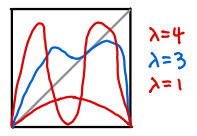
\includegraphics[width=4cm]{Immagini/Seconda_iterata_Logistica.png}
    \caption{Grafico di $T^2_\la$ al variare di $\la$.}
    \label{LogisticaIterata}
\end{figure}

\noindent
Cerchiamo di capire se $\Oc=\cpa{x_{\pm}(\la)}$ \`e un'orbita attrattiva:
\[(T_\la^2(x))'=T_\la'(T_\la(x))T'_\la(x),\]
da cui dopo dei conti
\[\abs{(T^2_\la)'(x_{\pm}(\la))}=\abs{4+2\la-\la^2},\]
quindi $\Oc$ \`e attrattiva se $\la\in [3,1+\sqrt 6]$ e repulsiva se $\la\in (1+\sqrt 6,4)$.
\vspace{0.25cm}

\noindent Possiamo graficare al variare di $\la\in [0,4]$ le orbite stabili (fattibile al computer in quanto stabili). 
Osserviamo dai risultati ottenuti che per $\la<1$ ci aspettiamo solo l'unico punto fisso $0$, poi per $\la\in(1,3)$ l'unico punto fisso attrattivo \`e $1-\la\ii$, poi per $\la\in (3,1+\sqrt 6)$ troviamo una orbita periodica attrattiva di periodo 2 e possiamo immaginarci di trovare ulteriori suddivisioni dell'intervallo rimanente dove l'orbita graficata ha periodo minimo variabile.

\begin{figure}[!htb]
    \centering
    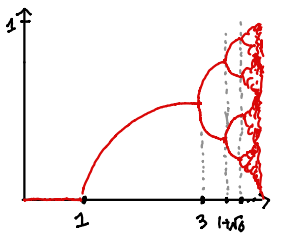
\includegraphics[width=7cm]{Immagini/Diagramma_biforcazione_logistica.png}
    \caption{Diagramma di biforcazione della mappa logistica. Sulle ascisse si succedono i valori di $\la$.}
    \label{DiagrammaBiforcazione}
\end{figure}
\noindent
Per ogni $\la$ fino ad un certo valore possiamo trovare $\Omega^\la$ invariante dato da un'orbita periodica ma per $\la\uparrow$ convergiamo verso un $\Omega^\infty$ invariante che non \`e un orbita periodica. $\Omega^\infty$ \`e uno \textbf{strange attractor}\footnote{Questo tipo di fenomeni dimostra che in genere lo studio delle orbite non \`e sufficiente. Per capire meglio questi sistemi dinamici \`e spesso utile definire misure.}.



\subsection{Mappa Tenda}

\begin{definition}[Mappa tenda]
Una funzione continua $T_a:[0,1]\to[0,1]$ si dice \textbf{tenda} se \`e della forma
\[T_a(x)=\begin{cases}
ax & 0\leq x< \frac12\\
a(1-x) & \frac12\leq x\leq 1
\end{cases},\quad 0\leq a\leq 2.\]
\end{definition}

\begin{example}[Insiemi invarianti per mappa tenda e mappa lineare]
Sia $T_a$ la mappa tenda come sopra e $T_b:[0,1]\to [0,1]$ la mappa lineare $T_b(x)=bx$ (poniamo $b\in [0,1]$).
\begin{figure}[!htb]
    \centering
    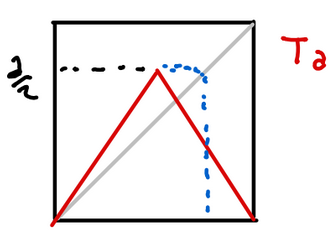
\includegraphics[width=4cm]{Immagini/Insieme_invariante_tenda.png}
    \caption{Grafico di una mappa tenda}
\end{figure}
Graficamente osserviamo che $T_a([0,1])=[0,\frac a2]$, quindi $[0,\frac a2]$ \`e positivamente invariante, ma \`e invariante solo se $a\geq 1$.
\begin{figure}[!htb]
    \centering
    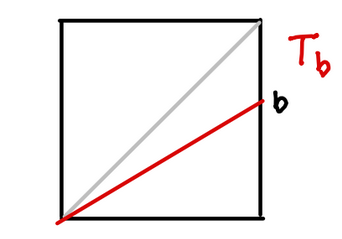
\includegraphics[width=4cm]{Immagini/Insieme_invariante_lineare.png}
    \caption{Grafico di una mappa lineare}
\end{figure}
Osserviamo che $T_b([0,1])=[0,b]$, quindi $[0,b]$ \`e positivamente invariante, ma \`e invariante solo per $b=1$.
\end{example}

\begin{example}[Dinamica della mappa tenda]
Sia $T=T_a$ la mappa tenda di parametro $a$. 
\begin{figure}[!htb]
    \centering
    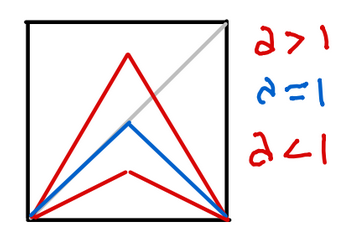
\includegraphics[width=4cm]{Immagini/Tipi_mappa_tenda.png}
    \caption{Grafico della mappa tenda per tre valori di $a$.}
\end{figure}

\noindent
Osserviamo graficamente che 
\[\text{Punti fissi}=\begin{cases}
\cpa{0} &a\in (0,1)\\
\spa{0,\frac12} &a=1\\
\cpa{0,\frac a{1+a}} &a>1
\end{cases}\]
Studiamo il comportamento di $0$ e $\frac a{1+a}$ (il secondo solo nel caso di $a\geq 1$)
\setlength{\leftmargini}{0cm}
\begin{itemize}
\item[$\boxed{0}$] Osserviamo che
\[\abs{T'(0)}=a,\]
quindi $0$ \`e iperbolico per $a\neq 1$. L'attrattivit\`a dipende dal segno di $a-1$.
\item[$\boxed{\frac a{1+a},\ a\geq 1}$] Anche in questo caso
\[\abs{T'\pa{\frac a{1+a}}}=a,\]
quindi questo punto \`e repulsivo per $a>1$ mentre per $a=1$ il punto non \`e iperbolico.
\end{itemize}
\setlength{\leftmargini}{0.5cm}
Studiamo la dinamica al variare di $a$
\setlength{\leftmargini}{0cm}
\begin{itemize}
\item[$\boxed{a=1}$] Per $x\in \spa{0,\frac12}$ si ha che $x$ \`e un punto fisso. Se $x\in (\frac12,1]$ allora $T(x)\in [0\frac12)$, quindi i punti sono ``definitivamente fissi".
\item[$\boxed{a<1}$] L'unico punto fisso \`e $0$ e $\omega(x)=\cpa{0}$ per ogni $x$.
\item[$\boxed{a>1}$] Abbiamo due punti fissi, ma sono entrambi repulsivi. Proviamo a studiare l'iterata seconda
\begin{figure}[!htb]
    \centering
    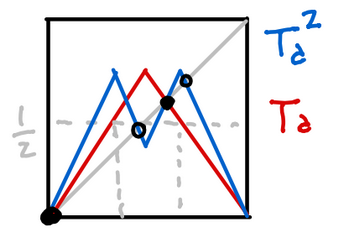
\includegraphics[width=4cm]{Immagini/mappa_tenda_iterata.png}
    \caption{Grafico della mappa tenda e della sua seconda iterata per $a>1$. In nero sono evidenziati i punti fissi di $T$ mentre con un cerchio sono evidenziati i punti di periodo minimo $2$ (visti come punti fissi di $T^2$).}
\end{figure}

Notiamo che se $x_1$ \`e uno dei punti fissi di $T$ allora $\abs{(T^2)'(x_1)}=a^2>1$, quindi continuano ad essere repulsivi anche per $T^2$ (non esistono dunque orbite attrattive di periodo 2).
\end{itemize}
\setlength{\leftmargini}{0.5cm}
\end{example}
    
\begin{remark}[Esempio di coniugio topologico]
La mappa logistica $T_4$ \`e coniugata topologicamente alla mappa tenda $T_2$.
\end{remark}
\begin{proof}
Basta considerare $\vp:[0,1]\to [0,1]$ data da
\[\vp(x)=\sin^2\pa{\frac\pi2x}\]
e notare che $\vp\circ T_2=T_4\circ \vp$\footnote{entrambe le composizioni assumono il valore $\sin^2(\pi x)$. Ricordiamo che $2\sin(\theta)\cos(\theta)=\sin(2\theta)$.}.
\end{proof}

\section{Miscellanea}
\begin{example}[Oscillatore armonico perturbato]
Sia $f:\R\to \R$ una funzione $1$-periodica. Immaginiamo una palla che rimbalza su un piatto la cui altezza varia come $f$. Per semplificarci la vita possiamo immaginare che l'urto avvenga sempre in $x=0$, tanto l'unica cosa che conta \`e $\dot f$ (l'impulso). Siano $t_0,t_1,\cdots,t_n$ i tempi di urto ($t_0=0$) e siano $v_0,\cdots,v_n$ le velocit\`a dopo l'urto. Conoscendo questi dati possiamo ricostruire tutta la dinamica.
\[T:\funcDef{[0,+\infty)\times (0,+\infty)}{[0,+\infty)\times (0,+\infty)}{(t_{n},v_n)}{(t_{n+1},v_{n+1})}.\]
Calcoliamo
\[\begin{cases}
t_{n+1}=t_n+h(v_n)\\
v_{n+1}=v_n+2\dot f(t_{n+1})
\end{cases},\quad h(v_n)=\frac 2gv_n\]
Osserviamo inoltre che
\[T(t_n+1,v_n)=(t_n+1+h(v_n), v_n+2\dot f(t_n+1 h(v_{n+1})))=T(t_n,v_n)+(1,0),\]
quindi in realt\`a possiamo considerare $S^1$ al posto di $[0,+\infty)$ per i tempi.\\
Questo sistema \`e difficile da trattare e presenta molti problemi aperti.
\end{example}

\begin{definition}[Ferro di cavallo di Smale]
Sia $\la>2$. Una trasformazione del tipo \textbf{Ferro di cavallo di Smale} \`e definita intuitivamente come segue
\begin{figure}[!htb]
    \centering
    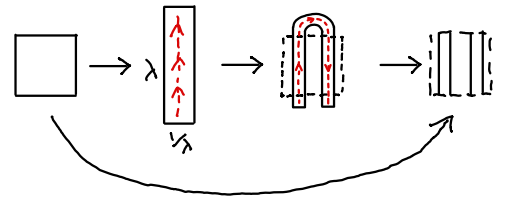
\includegraphics[width=11cm]{Immagini/Ferro_di_cavallo_di_Smale.png}
\end{figure}
\end{definition}




